%for a more compact document, add the option openany to avoid
%starting all chapters on odd numbered pages
\documentclass[12pt]{cmuthesis}

% This is a template for a CMU thesis.  It is 18 pages without any content :-)
% The source for this is pulled from a variety of sources and people.
% Here's a partial list of people who may or may have not contributed:
%
%        bnoble   = Brian Noble
%        caruana  = Rich Caruana
%        colohan  = Chris Colohan
%        jab      = Justin Boyan
%        josullvn = Joseph O'Sullivan
%        jrs      = Jonathan Shewchuk
%        kosak    = Corey Kosak
%        mjz      = Matt Zekauskas (mattz@cs)
%        pdinda   = Peter Dinda
%        pfr      = Patrick Riley
%        dkoes = David Koes (me)

% My main contribution is putting everything into a single class files and small
% template since I prefer this to some complicated sprawling directory tree with
% makefiles.

% some useful packages
\usepackage{times}
\usepackage{fullpage}
\usepackage{graphicx}
\usepackage{amsmath}
\usepackage{cite}
\usepackage{multirow}
\usepackage[numbers,sort]{natbib}
\usepackage[pageanchor=true,plainpages=false, pdfpagelabels, bookmarks,bookmarksnumbered,
%pdfborder=0 0 0,  %removes outlines around hyper links in online display
]{hyperref}
\usepackage{rotating}
\usepackage{setspace}
\usepackage{subfigure}
\usepackage{titlesec}
\DeclareMathOperator*{\argmin}{arg\,min}
\newcommand\addtag{\refstepcounter{equation}\tag{\theequation}}
\titleformat{\chapter}[hang] 
{\normalfont\LARGE\bfseries}{\chaptertitlename\ \thechapter:}{1em}{}

% Approximately 1" margins, more space on binding side
%\usepackage[letterpaper,twoside,vscale=.8,hscale=.75,nomarginpar]{geometry}
%for general printing (not binding)
\usepackage[letterpaper,twoside,vscale=.8,hscale=.75,nomarginpar,hmarginratio=1:1]{geometry}

% Provides a draft mark at the top of the document. 
\draftstamp{\today}{DRAFT}

\begin {document} 
\frontmatter

%initialize page style, so contents come out right (see bot) -mjz
\pagestyle{empty}

\title{ %% {\it \huge Thesis Proposal}\\
{\bf Characterizing Guitar Strings as Inharmonicity Trajectories for Automatic Tablature Transcription}}
\author{Jonathan Michelson}
\date{May 2017}
\Year{2017}
\trnumber{}

\committee{
Dr. Richard Stern, Dr. Thomas Sullivan \\
}

\support{}
\disclaimer{}

% copyright notice generated automatically from Year and author.
% permission added if \permission{} given.

%\keywords{Stuff, More Stuff}

\maketitle

%\begin{dedication}
%For my dog
%\end{dedication}

\pagestyle{plain} % for toc, was empty

%% Obviously, it's probably a good idea to break the various sections of your thesis
%% into different files and input them into this file...

%\doublespacing
\begin{abstract}
We propose and evaluate an additional inharmonicity-based method for automatic tablature transcription using only audio. First, we characterize each guitar string as the linear relation between its log-inharmonicity and fundamental pitch. Then we use these learned trajectories or regressions to classify string labels of unseen guitar notes: the system assigns to a pitch the label of the line which approximates the note's estimated inharmonicity with minimal residual. Given the tuning of the guitar that produced the unseen note, we infer its associated tablature, which allows for further string classification refinement by rejecting and reassigning implausible fret assignments. Average F1-scores achieved with this system for classical, acoustic, and electric guitars in the RWC instruments dataset were $0.92$, $0.94$, and $0.79$ respectively, rivaling performance of existing inharmonicity-based systems. We also derive and evaluate an inharmonicity compensation feature to allow for transcription of arbitrarily-tuned guitars, provided the tuning is known. With this enhancement, our average system accuracy improves by $7\%$ on alternate-tuned guitars, compared to performance with no tuning compensation.

\end{abstract}
%\singlespacing

\begin{acknowledgments}
Rich Stern
Tom Sullivan
Che-yuan Liang, Raymond Xia
Hodgkinson -- for sharing MAT algorithm
Abesser,Barbancho -- for their helpful correspondence
\end{acknowledgments}



\tableofcontents
\listoffigures
\listoftables

\mainmatter

%% Double space document for easy review:
%\renewcommand{\baselinestretch}{1.66}\normalsize

% The other requirements Catherine has:
%
%  - avoid large margins.  She wants the thesis to use fewer pages, 
%    especially if it requires colour printing.
%
%  - The thesis should be formatted for double-sided printing.  This
%    means that all chapters, acknowledgements, table of contents, etc.
%    should start on odd numbered (right facing) pages.
%
%  - You need to use the department standard tech report title page.  I
%    have tried to ensure that the title page here conforms to this
%    standard.
%
%  - Use a nice serif font, such as Times Roman.  Sans serif looks bad.
%
% Other than that, just make it look good...
\doublespacing
\noindent
\chapter{Introduction} 
The guitar is a popular musical instrument whose family comprises a diverse collection of stringed instruments. Its most prominent classes are the acoustic, classical, and electric guitars, and intraclass variation in characteristics such as body shape, string material, and amplification mode is high. Despite this diversity, the majority of guitar configurations have six strings tuned to $E2$ ($82$Hz), $A2$ ($110$Hz), $D3$ ($147$Hz), $G3$ ($196$Hz), $B3$ ($247$Hz), and $E4$ ($330$Hz). To play, a performer presses these strings with one hand against the neck's metal frets, each of which increase the string's pitch by one half-step, while strumming or plucking them with the other hand. Guitars typically have upwards of 20 frets, allowing for versatile musical passage realizations along the fretboard.

A consequence of this is liberal pitch overlap between neighboring strings. Conventional music scores that represent passages as notes and chords therefore fail to communicate fretboard position. This ambiguity renders scores unfit for guitar students trying to learn more skillful placement of scales and arpeggios, or for enthusiasts trying to decrypt the fretboard positions used on recordings of virtuosic players' riffs. Figure~\ref{fig:score-tabs} illustrates this ambiguity.

Tablature, on the other hand, is an alternative music notation that doesn't suffer from the one-to-many mapping of scores. The staff, instead of representing pitch as in classical scores, depicts a birds-eye view of the guitar neck from the performer's perspective. Each of the six horizontal lines signify a corresponding string on the guitar, and numbers on each line specify the fret to be played. Time progresses from left to right as in scores. 

\begin{figure}[h] 
\label{fig:score-tabs}
\centering
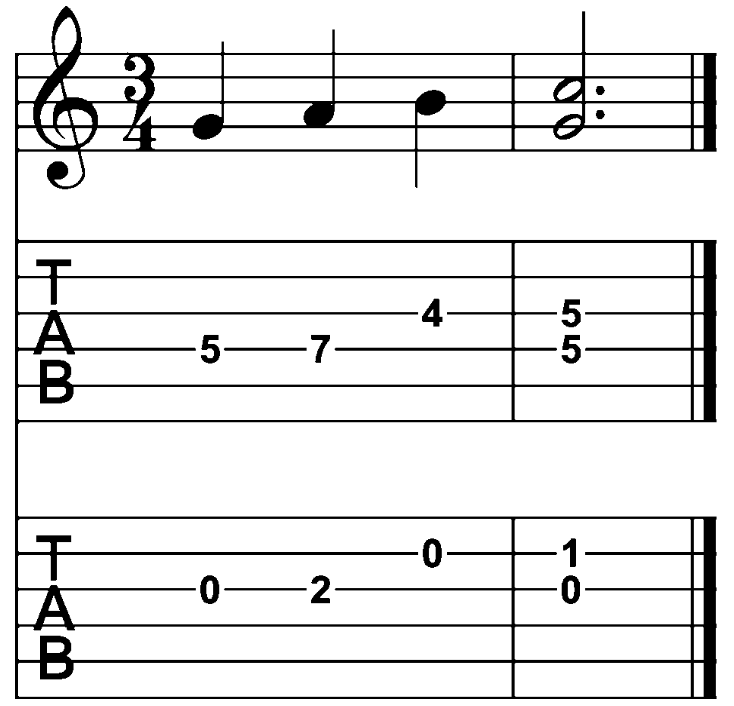
\includegraphics[scale=0.8]{score-tabs}
\caption{Musical score and two identical realizations of that score in tablature notation. Figure taken from~\cite{barbanchoi2012}.}
\end{figure}

Tablature (tabs for short) is widely popular for a number of likely reasons. Its accessibility and intuition are attractive to those without formal musical training; learning from a pictorial representation of one's instrument must seem more attractive to beginners than learning musical theory foundations and decoding scores. And because tabs are easily encodable and interpretable with simple ASCII characters, authoring them isn't limited to those with knowledge of any sort of tab-specific generation program, unlike with scores.~\cite{macrae2010}.

Accurate tablature transcription is a fairly tedious task, however. Dependable tabs containing few errors typically require a seasoned musician's careful listening to an audio recording, and possibly video recordings if available too. Reliable automation of this transcription task would benefit the guitar student community by expediting quality tab generation and unearthing fretboard positions of guitar riffs in songs for which accurate tabs don't yet exist. Recent technologies proposed to encourage proliferation of accessible tab transcription systems, such as web framework Robotaba~\cite{burlet2013}, demonstrate a desire among MIR researchers to see this theoretically mature but practically nascent field mature into student-benefitting applications. Closely related to tab transcription is the task of string classification: producing the correct tablature is straightforward if the guitar's tuning is known and the correct string labels are identified. 

In the next chapter, we survey previous work in the field of automatic tablature transcription, and highlight the feature known as inharmonicity. Then in Chapter~\ref{method}, we motivate inharmonicity's suitability for the string discrimination task, looking at Barbancho's work as an example. We transition to discussing the novel approach of our system. Chapter~\ref{experiments} contains descriptions and results of our experiments, and the discussion Chapter~\ref{discussion} regards an anlaysis of the results, shortcomings, and remaining work. We summarize this work in our final chapter.

\noindent
\chapter{Previous Work}
\section{Automatic Tablature Transcription}
\subsection{Graph Search Methods}
A popular framework for the stringed-instrument transcription task, introduced by Sayegh~\cite{sayegh} for both transcription and fingering problems, is that of weighted directed graphs that capture all plausible sequences of fretboard positions for a given musical passage. Edge weights in the graph are typically informed by mechanical or musical desirability of the fretboard sequences implied by the vertex transitions. Radicioni~\cite{radicioni} used this graph paradigm to obtain optimal tablatures from music scores. Yaezawa~\cite{yaezawa} extracted pitch and melody information from guitar recordings, and computed an optimal fingering based on plausible multipitch estimation results. Burlet~\cite{burlet} developed a polyphonic extension to monophonic optimal search algorithms. Radisavljevic~\cite{radisav2004} proposed a method to learn the optimal weights on the graph given optimal tablature.

\subsection{Machine Learning Solutions}
A number of teams have used machine learning techniques to ascertain fretboard position or related parameters. Gagnon~\cite{gagnon2003} proposed using neural networks on scores to deduce general fretboard region position and number of strings playing, while Tuohy~\cite{asdf} used a genetic algorithm on scores to obtain tablature. Barbancho et al. ~\cite{barbancho2009} attempted guitar string classification with a Fisher linear discriminant using a multitude of time and frequency-domain features. Abesser~\cite{abesser2012}, Dittmar~\cite{dittmar2013}, and Kehling~\cite{kehling2014} achieve good string transcription performance after training an SVM on standard-tuning guitar audio and using a slew of partials-related features. Burlet~\cite{} developed a deep belief network that achieved fretboard transcription from audio.

\subsection{Multimedia Approaches}
Some researchers have explored usage of media other than audio or musical information (i.e., scores). Ogrady~\cite{} exploited hexaphonic pickups and matrix factorization of their output to record fretboard positions. Paleari~\cite{}, Burns~\cite{}, and Kerdvibulvich~\cite{} extract tablature from video recordings using image processing and computer vision techniques.

\subsection{The Partial Coincidence Tally (PCT) Method}
One system in particular served as inspiration for this work. Barbancho~\cite{barbanchoi2012} realized the discriminative potential of a singular feature known as inharmonicity, and devised an algorithm that exclusively used inharmonicity to achieve impressive transcription results using only audio. We discuss inharmonicity in detail and methods for its estimation in the next two sections. Barbancho's method, which we refer to as the "partial coincidence tally" method, is also given a more thorough treatment later in Chapter~\ref{method}.

We were particularly interested in the PCT method for a number of reasons. Firstly, its input is audio. This is important because other media are less -------; scores are inaccessible to novices, while video recordings somewhat nullify the need for tablature ascertainment in the first place. Among the most interesting use cases for an automatic tab transcription system are certainly direct audio-to-tab capability. Other inputs, like scores or video footage of the guitar neck, are already levels of transcription that detracts from the novelty of such a system. Secondly, PCT is rooted in physics which allows for potential transcription of theoretically any fretboard position. Lastly, their method exclusively uses inharmonicity. Other systems that use inharmonicity~\cite{barbancho2009,abesser2012,dittmar2013,kehling2014} exploit additional features that are, in light of~\cite{barbanchoi2012}, superfluous regarding the discriminative information they contribute. 

\section{Inharmonicity Motivation}
To understand the motivation for this work, we first need to address the motivation behind inharmonicity as a feature itself. Inharmonicity is key in many string discrimination systems~\cite{barbanchoi2012,abesser2012,dittmar2013,kehling2014}. When an ideal string fixed at both ends is displaced, the restoring force that causes it to oscillate is its tension. However, for a real string with stiffness, its elasticity contributes to this restoring force~\cite{fletcher1962} which causes the frequencies of the modes of vibration to no longer be integer multiples of the fundamental. Instead, they're skewed upward according to: 
\begin{equation}
\label{eq:fk}
f_k = kf_{0}\sqrt{1+\beta k^2}
\end{equation}
where $f_k$ is the $k$th harmonic of fundamental $f_0$ and $\beta$ is the string's inharmonicity, defined by
\begin{equation}
\beta = \frac{\pi^3 Q d^4}{64 T l^2}. \label{eq:beta}
\end{equation}
In words, the inharmonicity $\beta$ of a vibrating string is a dimensionless quantity that depends on the string's Young's modulus $Q$, diameter $d$, tension $T$, and vibrating length $l$, and which scales the degree of deviation of the string's $k$th partial according to equation~(\ref{eq:fk}). See Figure~\ref{fig:skew}. Note that for an ideally harmonic string, $\beta = 0$ and~(\ref{eq:fk}) reduces to $f_k = kf_0$, aligning with intuition about harmonics' ideal locations in frequency as simply integer multiples of the fundamental.

\begin{figure}[!htbp]
\label{fig:skew}
\centering
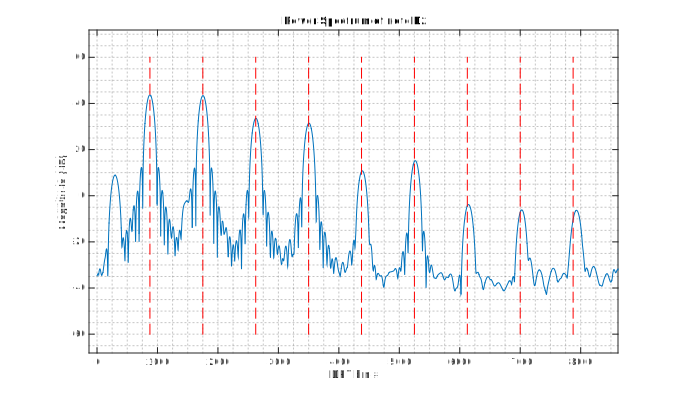
\includegraphics[scale=0.65]{skew}
\caption{Power spectrum of note D2 plucked on an electric guitar at string 5 and fret 5. Red dashed lines are drawn at integer multiples of the fundamental. Note the rightward skew of the measured partial peaks.}
\end{figure}

Inharmonicity's suitability for the string discrimination task can be understood through equation~(\ref{eq:beta}). The six strings of any guitar necessarily exhibit different combinations of $Q$, $d$, and $T$ due to varying thicknesses, material, and tuning. Each string therefore has an "inharmonic signature" which presumably distinguishes it from the others. Capturing the pattern of a string's inharmonicity variation along its frets should thus reveal sufficiently identifying information.

\section{Inharmonicity Estimation}
\label{lit-beta-est}
Empirical estimation of inharmonicity is itself a topic of research which merits a brief review. Using pitch extraction techniques to perform estimation was first attempted by Galembo in 1979 and 1986~\cite{galembo1979,galembo1987}. Several additional methods have been proposed since then. In 1994, Galembo~\cite{galembo1994} hypothesized a connection between partials-based fundamental pitch estimates and the degree of inharmonicity in a spectrum. They specifically investigated cepstral analysis and a variant of the harmonic product spectrum method applied to both synthetic tones and recorded piano notes. They found that, because these two techniques leverage periodicity in the frequency domain to produce their pitch estimates, inharmonicity influenced the quality of their estimates in a deterministic manner: more inharmonicity produced wider, less focused pitch estimates lobes, and from quantifying this relation an inharmonicity could be obtained.
 
 The same authors in~\cite{galembo1999} introduced another method in 1999, dubbed the inharmonic comb filter (ICF) method. To estimate a note's inharmonicity, they first applied sets of comb filters to the note's spectrum. The locations of the comb filters' notches were parametrized with a range of inharmonicity values that sufficiently sampled the note's expected inharmonicity range. The ICF whose inharmonicity best matched that of the note would produce the output with lowest spectral energy, since its notches best aligned with the inharmonic note partials. The inharmonicity parameter associated with this output-minimizing ICF was thus selected as the estimate.
 
Rauhala~\cite{rauhala2007} introduced an efficient procedure in 2007 that iteratively catalogued estimates of the partial frequencies' deviations and returned increasingly better estimates of the inharmonicity. The algorithm, aptly referenced as the partial frequency deviations (PDF) method, is initialized with a reasonable first estimate of inharmonicity, and then the note's spectrum is searched for partial peaks. Differences are measured between the locations of these discovered peaks and those of the expected peaks, and the aggregate deviation trend is used to refine the inharmonicity estimate -- a majority of positive differences implies the inharmonicity should be reduced, and a majority of negative differences implies the opposite.

In 2009, Hodgkinson~\cite{hodgkinson2009} proposed a yet more efficient and accurate algorithm, named median-adjustive trajectories (MAT). Their routine exploits the fact that inharmonicity can be estimated with any two partials and their corresponding indices in the harmonic series. Pairs of low-index partials are first considered, since they're minimally affected by inharmonic skew and therefore have high location reliability. With these initial inharmonicity estimates, additional partials are collected and used to refine the previous inharmonicity estimates, with which more partials are located, so on and so forth. MAT was the inharmonicity estimation routine employed in this work, and is discussed at length in Chapter~\ref{experiments}.

Three years later, Barbancho~\cite{barbanchoi2012} introduced another PFD-based approach as part of a guitar tablature transcription system. They started by cataloguing the first 10 partials' deviations, then fitting a polynomial to the PFD curve. They derived the relation between the polynomial's coefficients and the inharmonicity, and returned an initial inharmonicity estimate according to this derivation. Then using this inharmonicity to aid in their search for higher-index partials, they catalogued a larger number of partials' deviations than that of the first iteration, and performed the same polynomial fit and inharmonicity derivation routine. This would refine the inharmonicity estimate, allowing for increasing numbers of partials for which to search.

Also in 2012, Abesser~\cite{abesser2012} used parametric spectral modeling, again in the context of a guitar tablature transcription system. To estimate the inharmonicity of a plucked guitar note, they modeled each audio frame with the autoregressive (AR) filter that best approximated its spectral content. They obtained the poles' locations and the ideal harmonics' locations, and like Barnbancho~\cite{barbanchoi2012} fit the PFD curve with a polynomial from whose coefficients an inharmonicity estimate could be derived.



\noindent
\chapter{Characterizing Strings as Inharmonicity Trajectories}
\label{chap:method}
In this chapter, we present our automatic tablature transcription system in detail. We begin with the motivation for our approach, then present its various building blocks: the specific inharmonicity estimation algorithm we used, transformation of inharmonicity to log-inharmonicity, compensation for arbitrary tuning, learning log-inharmonicity trajectories, string classification using the learned trajectories, and the final tablature conversion and refinement process.
\section{Motivation}
Barbancho~\cite{barbanchoi2012} derived that inharmonicity varies in a deterministic manner with respect to fret positions along a given string. Specifically, they showed that the inharmonicity $\beta(s,n)$ of a note produced by string $s$ at fret number $n$ could be expressed in terms of the inharmonicity of the open-string note $\beta(s,0)$ according to:
\begin{equation} 
\label{eq:beta-traj}
\beta(s,n) = \beta(s,0)2^{\frac{n}{6}}
\end{equation}
In other words, the variation in inharmonicity along a given string can be expressed simply in terms of its open-note inharmonicity, effectively defining a restricted trajectory along which the inharmonicity must vary. Figure~\ref{fig:beta-trajectories-ag} illustrates these trajectories.

\begin{figure}[h] 
\label{fig:beta-trajectories-ag}
\centering
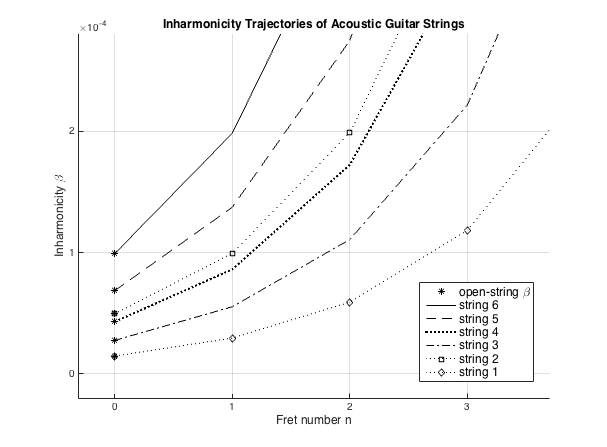
\includegraphics[scale=0.70]{beta-trajectories-ag}
\caption{Example inharmonicity trajectories of acoustic guitar strings. Only frets 0 (open-string) through 3 are shown. Observe the restriction to the exponential trajectory defined by equation~\eqref{eq:beta-traj}.}
\end{figure}

Recognizing this, they were able to successfully transcribe string and fret number of an unknown guitar note. Their system's essential mechanism was a similarity-determination routine $A(X,\hat{\beta}_s)$ that quantified the resemblance between an unknown note's spectrum $X$ and the expected inharmonicities $\hat\beta_s$ of candidate strings $s$ from which the note could have originated. First, to estimate an open-note's inharmonicity they followed the procedure described in section~\ref{lit-beta-est} in which they estimated its fundamental, then catalogued its partials' deviations from their ideal harmonic locations, and fit to them a polynomial from whose coefficients they derived the inharmonicity estimate. Next, they inferred the corresponding fret on which the note could be played for each candidate string, and used these string-fret candidate numbers in equation~\eqref{eq:beta-traj} to obtain expected inharmonicity values of the unknown note for each candidate string. In other words, they followed each candidate string's inharmonicity trajectory to arrive at an expected inharmonicity value at the appropriate fret. Lastly, they applied their similarity determination algorithm $A(X,\hat{\beta}_s)$, which went as follows. For each candidate fretboard position, they obtained the expected skewed frequency locations at which to find the inharmonic peaks, and searched the note's spectrum for them using search windows centered at those expected locations. They performed this search for a set number of peaks, all the while cataloguing their deviation from the search window centers. Their motivation was that the expected inharmonicity of the true fretboard position would produce a spectrum with inharmonic peaks that were measurably more coincident with the inharmonic peaks of the unknown note than were any of the imposter strings. They found that, indeed, the inharmonicity of the fretboard position on which the note was truly plucked yielded the largest number of coincident located peaks inside the spectral search window bounds, hence our name "partials coincidence tally" for their algorithm. Their work demonstrated the sufficiency of inharmonicity as a discriminating feature.

This work capitalizes further on their trajectory realization. Rather than zooming into fretboard positions' spectra to evaluate their candidacy, we propose characterizing each candidate string by its inharmonicity trend and classifying a note as belonging to the string whose inharmonicity trajectory evaluated at the note's fundamental best approximates the note's inharmonicity. In other words, our similarity routine is simply some error calculation $A'(\beta,\hat{\beta})$, discussed in detail in the next sections, between the note's inharmonicity $\beta$ and each candidate fretboard positions' predicted inharmonicity $\hat{\beta}$ for the note. This is an algorithmically simple approach, requiring merely inharmonicity estimation of the unknown note, inharmonicity trends of training guitars' strings, and an error measure. Additionally, this method is governed by the intuitive spatial constraint of inharmonicity trajectory: notes played on a given string can exhibit only a set of inharmonicities, so classifying based on a spatial metric like minimal residual from a regression makes physical sense.

\section{Inharmonicity Estimation}
The first step in our system is estimation of the inharmonicity of an unseen note. The algorithm we employed was the median adjustive trajectories (MAT) method~\cite{hodgkinson2009} proposed by Hodgkinson in 2009, and we present it here. At the core of this method is a recasting of the definition of inharmonicity in terms of any two partials and their indices. We can rearrange equation~\eqref{eq:fk} to express the fundamental $f_0$ in terms of the frequency $f_m$ of the $m$th partial and its index $m$ as
\begin{equation}
\label{mat6}
f_0 = \frac{f_m}{m\sqrt{1+\beta m^2}}.
\end{equation}
Next, we can substitute~\eqref{mat6} back into $f_0$ in equation~\eqref{eq:fk} to obtain
\begin{equation}
\label{mat7}
f_k = \frac{kf_m}{m\sqrt{1+\beta m^2}}\sqrt{1+\beta k^2}.
\end{equation}
Solving for $\beta$ yields
\begin{equation}
\label{mat8}
\beta = \frac{(f_k\frac{m}{k})^2-f_m^2}{k^2f_m^2-m^2(f_k\frac{m}{k})^2},
\end{equation}
which defines the inharmonicity of a note in terms of an arbitrary two partials $k$ and $m$ and their corresponding frequencies $f_k$ and $f_m$.

The MAT algorithm begins by locating partials 1 and 2 based on a user-input estimate of the fundamental. Searching for these partials is straightforward, since the skew effect of inharmonicity is low for small indices. From these locations,~\eqref{mat8} is used for every combination of the located partials (which for this first iteration, is only one) to obtain an array of $\beta$ estimates. The median of the $\beta$ array is returned as the composite $\beta$ estimate of this iteration, and this median together with the partials' locations are used in~\eqref{mat6} to obtain an array of revised $f_0$ estimates that contains as many elements as partials under consideration. Finally, the median of this $f_0$ array and the median of the $\beta$ array are used in equation~\eqref{eq:fk} to predict the frequency of the next partial for which to search, which is the third in this case. At succeeding iterations, the lengths of these $f_0$ and $\beta$ arrays grow longer (since both the number of partials, and therefore the number of combinations of partials pairs, increases), and the estimates which they contain grow increasingly more accurate. The algorithm is summarized in the flowchart in Figure~\ref{fig:mat-flowchart}, taken from ~\cite{hodgkinson2009}. MAT determines the ideal number of partials for which to search by finding the highest partial index that lies above the average level of the magnitude spectrum, and terminates once this partial index is reached. The result is an efficient and accurate inharmonicity estimation routine. 
\begin{figure}[!htbp] 
\label{fig:mat-flowchart}
\centering
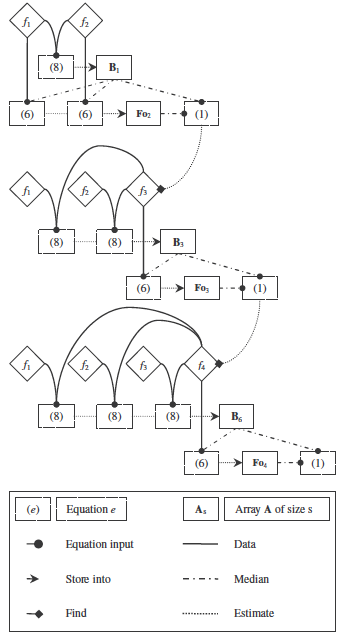
\includegraphics[scale=0.9]{mat-flowchart}
\caption{Median-adjustive-trajectory (MAT) method flowchart.}
\end{figure}

\section{Log-inharmonicity}
Next in our pipeline, we apply a log transformation to the estimated inharmonicity to make its variation with respect to MIDI pitch linear. This has the advantage of using simpler regression models for classification at later stages. If we reconsider equation~\eqref{eq:beta-traj} in terms of MIDI pitch number $m$ instead of fret number $n$, we obtain
\begin{equation}
\beta(s,m) = \beta(s,m_{os})2^{\frac{m-m_{os}}{6}},
\end{equation}
where $m_{os}$ is the open-string pitch of string $s$. The exponential trajectory is maintained since incrementing both fret number and MIDI pitch number accomplishes an equivalent increase in fundamental frequency. Figure~\ref{fig:beta-v-midi} illustrates the trajectories in terms of MIDI pitches.

\begin{figure}[h] 
\label{fig:beta-v-midi}
\centering
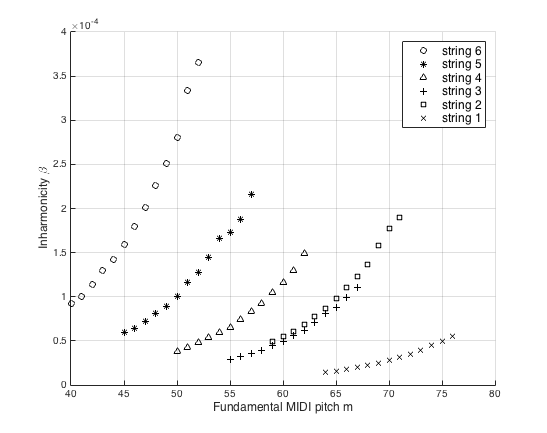
\includegraphics[scale=0.7]{beta-v-midi}
\caption{Inharmonicity estimates for frets 0-12 on strings 1-6 of RWC acoustic guitar 111AG. Note the exponential trajectory as in Fig.~\ref{fig:beta-trajectories-ag} and the increased segregation since notes and their inharmonicities are now plotted against their fundamental instead of their fret number.}
\end{figure}

Now if we consider the log-inharmonicity $\beta_{l}(m)$, we see that
\begin{equation}
\beta_l(m) = \log_2\beta(s,m) = \log_2[\beta(m_{os})2^{\frac{m-m_{os}}{6}}]
\end{equation}
\begin{equation}
\beta_l(m) = \log_2\beta(m_{os}) + \frac{m-m_{os}}{6}
\end{equation}
\begin{equation}
\beta_l(m) = (\log_2\beta(m_{os})-\frac{m_{os}}{6}) + (\frac{1}{6})m,
\end{equation}
where string $s$ has been dropped from the notation since we're looking only at variation along a fixed string. Substituting $w_0$ for $\log_2\beta(m_{os})-\frac{m_{os}}{6}$ and letting $w_1 = \frac{1}{6}$, we obtain the familiar linear form
\begin{equation}
\label{eq:linear-traj}
\beta_l(m) = w_0 + w_1m,
\end{equation}
showing us that the log-inharmonicity trajectory of a given string varies linearly with respect to MIDI pitch. See Figure~\ref{fig:log-beta-v-midi}. This relationship also holds for fret number, but fundamental pitch is a more likely and generic feature to have been estimated, and consequently is more relevant to consider here.

\begin{figure}[!htbp] 
\label{fig:log-beta-v-midi}
\centering
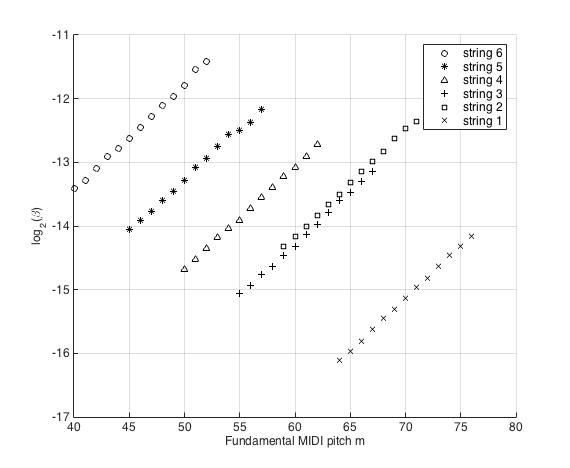
\includegraphics[scale=0.7]{log-beta-v-midi}
\caption{Log-inharmonicity estimates for same frets, strings, and guitar as Fig.~\ref{fig:beta-v-midi}}
\end{figure}

\section{Tuning Compensation}
After transforming our data into log-inharmonicity and MIDI pitch space, we apply a tuning compensation feature step if the test guitar is known to be in alternate-tuning. In this section, we derive the straightforward adjustment and explain how it is incorporated into our system. 

Though standard tuning is the most common pitch configuration of six-string guitars, there exist numerous other tunings in which performers often play. Aside from altering the musicality of the instrument, alternate tunings complicate the transcription process by introducing uncertainty about the open-string pitches. They distort inharmonicity-based methods, since the tensions $T$ of alternately-tuned guitar strings differ from those in standard-tuned strings, thereby affecting estimation of the inharmonicity. 

Current string classification systems don't address this degree of freedom. The method proposed by Barbancho~\cite{barbanchoi2012} is technically tuning-invariant, but would require access to recordings of the alternately-tuned test guitar's open strings and so isn't considered a classifier here. Other supervised learning systems~\cite{kehling2014, dittmar2013, abesser2012} are trained and evaluated only on standard-tuning guitars.

A possible approach to augment inharmonicity-based string classifiers with tuning-invariant performance is to simply introduce a scaling factor on the expected inharmonicity, or equivalently an additive factor on the expected log-inharonicity. The fundamental frequency $f_0$ of an ideal vibrating string is related to its tension $T$ according to
\begin{equation}
f_0 = \frac{1}{2L}\sqrt{\frac{T}{\mu}}
\end{equation}
where $L$ is string length and $\mu$ is its density. From this, we can see that
\begin{equation}
T \propto f_0^{2}.
\end{equation}
Recognizing that for a change in fundamental pitch of $\Delta m$ semitones, the equivalent change in frequency is $2^{\frac{\Delta m}{12}}$, we see that the proportional change in tension (with all other factors constant) is
\begin{equation}
T \propto 2^{\frac{\Delta m}{6}}f_0^2.
\end{equation}
The resulting log-inharmonicity of this new open-string note with pitch $m_{os}' = m_{os}+\Delta m$, with original open-string pitch $m_{os}$, is therefore
\begin{equation}
\log_2\beta(m_{os}') = \log_2[ \frac{\pi^3 Q d^4}{64 T l^2}(2^{-\frac{\Delta m}{6}})].
\end{equation}
\begin{equation}
\label{eq:delta-beta}
\log_2\beta(m_{os}') = \log_2\frac{\pi^3 Q d^4}{64 T l^2} - \frac{\Delta m}{6}.
\end{equation}
Substituting~\eqref{eq:delta-beta} into $w_0$ from equation~\eqref{eq:linear-traj} to obtain the new intercept term $w_0'$, we get
\begin{equation}
w_{0}' = \log_2{\beta}(m_{os}') - \frac{m_{os}'}{6}
\end{equation}
\begin{equation}
w_{0}' = (\log_2\frac{\pi^3 Q d^4}{64 T l^2} - \frac{\Delta m}{6}) - \frac{m_{os}+\Delta m}{6}
\end{equation}
\begin{equation}
\label{eq:3.17}
w_{0}' = \log_2\frac{\pi^3 Q d^4}{64 T l^2} - \frac{m_{os}}{6} - \frac{\Delta m}{3}
\end{equation}
\begin{equation}
\label{eq:3.18}
w_{0}' = w_0 - \frac{\Delta m}{3}.
\end{equation}
The slope coefficient $w_1 = -\frac{m}{6}$ is independent from ${\Delta m}$, so the affected log-inharmonicity trajectory of this alternately-tuned string is therefore
\begin{equation}
\label{eq:3.19}
\beta'(m) = w_0' + w_1'm
\end{equation}
\begin{equation}
\label{eq:3.20}
\beta'(m) = w_0 + w_1m - \frac{\Delta m}{3}.
\end{equation}
In words, equation~\eqref{eq:3.20} tells us that the effect of a string's alternate tuning is simply addition of a bias term $\frac{-\Delta m}{3}$ to the log-inharmonicity, where $\Delta m$ is the semitone deviation from standard tuning. We should thus be able to compensate our predictive trajectories to arbitrarily-tuned guitars, provided we're given the alternate tuning in which the unseen notes are being performed. As can be seen in Figure~\ref{fig:tuning-eg} when one string on the standard-tuned electric guitar is modified using equation~\eqref{eq:3.20}, the predictive alternate-tuning regression aptly captures the trend of the alternate-tuning inharmonicity. This is a straightforward modification for any inharmonicity-exploiting classifier, and we report our results with this modification in the next chapter.
\begin{figure}[!htbp] 
\label{fig:tuning-eg}
\centering
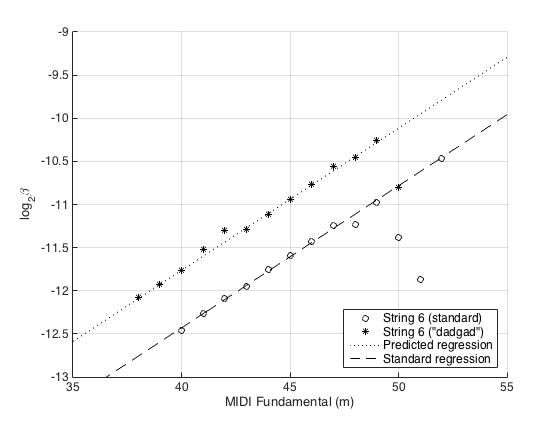
\includegraphics[scale=0.75]{tuning-eg}
\caption{Effect of alternate tuning on an electric guitar's log-inharmonicities. The circles are log-inharmonicity estimates of frets 0-12 on string 6 of RWC electric guitar EG131 in standard tuning, and the dashed line is their bisquare-weighted regression. The asterisks are log-inharmonicity estimates for the same frets, string, and guitar, but tuned two semitones down. The dotted line passing through them is the \textit{predicted} regression obtained by applying equation~\eqref{eq:3.20} to the dashed line.}
\end{figure}

\section{Learning Inharmonicity Trajectories}
We next need to train our system to understand strings' typical log-inharmonicity trajectories. There are two methods we use to do this. The first, which we call \textit{theoretical} trajectory determination, is the method Barbancho employed, so we use this for comparison of our system to theirs. For each guitar, we collect the six notes labeled with fret 0 (i.e. played open-string) from its recordings, and estimate their inharmonicities. To obtain a more robust estimate, we take the string-wise median of these estimates for our final six open-string inharmonicities. Our line trajectories are then simply those defined by equation~\eqref{eq:linear-traj}. 

%The coefficient vector $\mathbf{w}$ is $[w_0, w_1]^T$, with $w_0$ and $w_1$ as defined before. The independent variable vector $\mathbf{x}$ remains $[1, m]^T$, as discussed in the previous paragraph. The predicted inharmonicity $\hat{\beta}$ reduces to an evaluation of the linear function $\beta(m) = \mathbf{w}^T\mathbf{x}$ at the unknown note's fundamental pitch $m$, and it is these evaluations that are used in~\eqref{eq:classify} to classify strings.

The other method we use is linear regressions for obtaining \textit{empirical} log-inharmonicity trajectories. This is one of the novel features of this work. Regressing log-inharmonicities of notes against their pitches could capture a more fitting trajectory than the strictly theoretical trajectories obtained from equation~\eqref{eq:linear-traj}. In this method, we collect all notes with common string labels in our training data, and we perform linear regression of their log-inharmonicities $\beta$ against their fundamental pitches $m$ (in MIDI note number format). We do this for each string label. Let $s \in \{1,2,3,4,5,6\}$ be the string label to which each training note is assigned, and $N_s$ be the number of notes we have belonging to string label $s$. If we let $\mathbf{x}_s^{(i)} = [1, m_s^{(i)}]^T$ represent the $i$th note with fundamental pitch $m^{(i)}$ belonging to string $s$ , and $\beta_s^{(i)}$ be the log-inharmonicity of the $i$th note belonging to string $s$, we can solve
\begin{equation}
\label{lin-reg}
\mathbf{w}_s = \argmin_{\mathbf{w}}{\sum_{i=1}^{N_s}{(\beta^{(i)}_s - \mathbf{w}^T\mathbf{x}^{(i)}_s)^2}}
\end{equation}
which yields the weight vector $\mathbf{w}_s$ that minimizes the sum of squared error between the measured and predicted inharmonicities of the notes belonging to string $s$. Figure~\ref{fig:traj-v-reg} illustrates the differences between the trajectory and regression approaches.

\begin{figure}[!htbp] 
\label{fig:traj-v-reg}
\centering
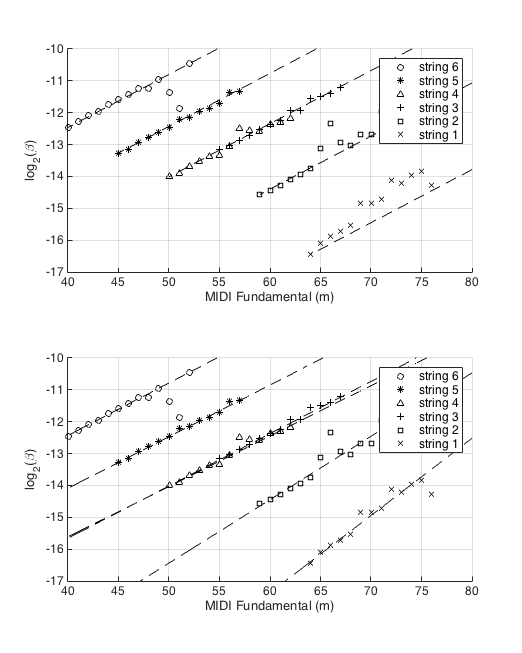
\includegraphics[scale=0.75]{traj-v-reg}
\caption{Comparison of string characterization approaches for our recorded Fender Telecaster. Top: inharmonicity \textit{trajectories}. Note how each line begins precisely at the first marker of each string (i.e. the open-string note) and continues along a trajectory that ignores empirical inharmonicity estimates. String 1 most clearly shows this. Additionally, the trajectories for strings 3 and 4 are effectively co-linear and therefore indiscriminible. Bottom: inharmonicity \textit{regressions}. Each regression was obtained by minimizing the bisquare weighted error of the string's residuals, so the lines more closely follow the empirical inharmonicity scatterplot estimates.}
\end{figure}

Mistakes in the inharmonicity estimation routine would sometimes produce outliers that deviated substantially from the linear trajectory model, and which disproportionately skewed the regressions. For this reason, we rather performed a bisquare weighted linear regression, instead of the standard unweighted regression in~\eqref{lin-reg}, to empirically approximate the log-inharmonicities. Bisquare weighting is a robust linear regression procedure that minimizes a weighted sum of squares that de-emphasizes outliers. The iterative procedure works as follows. First, a regular least squares fit is obtained. Then, the standardized adjusted residuals are computed according to
\begin{equation}
u = \frac{r_i}{Ks\sqrt{1-h_i}},
\end{equation}
where $r_i$ are the plain residuals, $h_i$ are the leverages, $K = 4.685$ is a tuning constant, and $s$ is the robust variance, which is equal to $M/0.6745$ where $M$ is the median absolute deviation of the residuals. Next, the robust weights are computed according to
\begin{equation}
w_i = \begin{cases}
(1-u_i^2)^2, & |u_i| < 1\\
0, & |u_i| \geq 1\\
\end{cases}
\end{equation} 
The process is repeated, iteratively improving the weights until the fit converges~\cite{matlab}. The Matlab robustfit routine was used to implement this.

\section{String Classification}
The next step is to use these learned string trajectories to classify unknown notes. Since these trajectories tell us how to expect different strings' inharmonicities to vary with respect to pitch, we think of string classification in this context as simply determining which trajectory or line best approximates the unseen note's inharmonicity estimate. To this end, we simply assign a note to the trajectory that minimizes the reconstruction error. 

Other decision functions were considered before deciding on residual minimization. We considered using a two-dimensional Euclidean distance metric, but ultimately steered away because it wasn't true to the physical phenomenon -- expected inharmonicity on a fixed string should be a function of only one variable, namely pitch, so incorporating an additional degree of freedom seems inappropriate. Indeed, one can easily imagine situations where the Euclidean distance between a note's inharmonicity estimate and an erroneous string is smaller than the one-dimensional residual between it and its true string, thereby producing an incorrect string classification. 

We also considered a probabilistic decision function. Because, for linear regression, minimizing the residual sum-of-square error of the data is equivalent to maximizing the likelihood of the data if its assumed the data was generated by Gaussian distributions with means centered at the regression line, we also attempted a probabilistic, or "soft" residual classifier. Unseen notes were assigned to the line from which it was most probably generated, given the lines' means and variances. The term "soft" arises from the fact that points are no longer necessarily assigned to the closest line -- the decision is evaluated strictly on probabilistic terms. We ultimately avoided this method, however, because our system was suffering from precision issues. The variances of the robust weighted regressions would consistently be tens or hundreds of orders of magnitude smaller than the distances to some outlier inharmonicities. The system would then incorrectly classify these outliers because of insufficient resolution. A workaround wasn't implemented because this, too, didn't quite fit the mechanism by which these inharmonicities were being produced in reality. Inharmonicity outliers were strictly due to inharmonicity estimation mistakes, not a physical phenomenon in the guitar, so it didn't seem appropriate to incorporate this into our model.

We thus settled on minimizing the residual error, which is explained here. We take the $n$th note in our test set, characterized by tuple $(m^{(n)},\beta^{(n)})$ where $m^{(n)}$ is its MIDI pitch number and $\beta^{(n)}$ is its inharmonicity. We'd like to transform this into another tuple $(s^{(n)},f^{(n)})$ corresponding to the appropriate string and fret to which this unknown note should be assigned. We straightforwardly assign to $s^{(n)}$ the index $j$ of the linear coefficients $\mathbf{w}_j$ whose predicted inharmonicity $\hat\beta_j$ approximates the measured inharmonicity $\beta^{(n)}$ with least error. More formally, we solve 
\begin{equation}
\label{eq:classify}
s^{(n)} = \argmin_{j}{(\beta^{(n)} - \hat{\beta}_{j})^2}
\end{equation}
where $\hat\beta_j$ is the inharmonicity prediction of string $j$, given by
\begin{equation}
\hat{\beta}_{j} = \mathbf{w}_{j}^T\mathbf{x}^{(n)}.
\end{equation}
Here, $\mathbf{x}^{(n)} = [1, m^{(n)}]^T$ to account for a y-intercept term. Figure~\ref{fig:classify} graphically illustrates this process.

\begin{figure}[!htbp] 
\label{fig:classify}
\centering
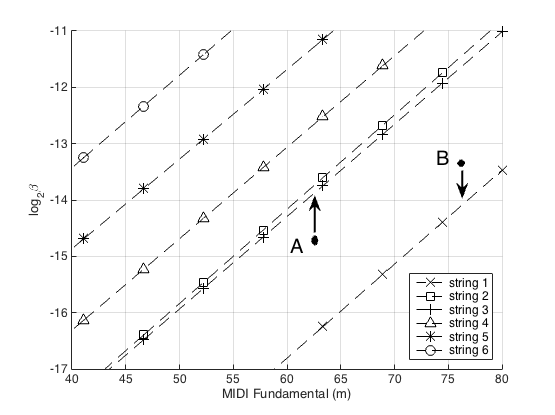
\includegraphics[scale=0.75]{classify}
\caption{Classifying two new notes A and B using learned log-inharmonicity characterizations. Dashed lines are actual learned regressions for RWC acoustic guitar AG091. Note A with fundamental pitch 62 is assigned to string 3, since its line characterization is closest to A's inharmonicity estimate. The residual of note B, with fundamental pitch 76, is smallest with respect to string 1, so it's assigned to that string under the least-square-error decision of equation~\eqref{eq:classify}.}
\end{figure}

Occasionally, outlier inharmonicity estimates would throw off this classification scheme. To combat this, we employed frame aggregation, a refinement technique used by~\cite{abesser2012}. In frame aggregation, inharmonicities of multiple audio windows are estimated and classified individually, then the multiple results are aggregated into a compound final decision. In essence, it's a form of averaging that relies on the theoretically low probability that consecutive inharmonicity estimates will all be outliers; the more probable stable estimates will contribute to a more reasonable aggregate string decision. For each frame $r$ in an $F$-frame aggregation of a note, we obtain the string-wise distances $\mathbf{d_r} = [d_1,d_2,d_3,d_4,d_5,d_6]^T$ between its log-inharmonicity estimate and all possible strings $s$. Then, we simply sum the distances $\mathbf{d_r}$ over all frames and select the string whose aggregate distance is minimal:
\begin{equation}
\hat{s} = \argmin_{s\in\{1,2,3,4,5,6\}}\sum_{r=1}^{F} \mathbf{d_r}.
\end{equation}
The result is a tamer inharmonicity estimate and a slight boost in classification accuracy. For our system, we used 5 abutting frames, each 100ms long, which start at the detected onset of a note. Onsets were obtained through automated detection, the details of which are beyond the scope of this work but are cited for reference~\cite{bello2005,dixon2006}.

\section{Tablature Conversion and Refinement}
The final step is transformation of the string classifier output into tablature notation. Because the classifier outputs are string numbers, we still need to infer notes' fret positions. This is a trivial task provided we know the tuning $\mathbf{t} = [m_1, m_2, m_3, m_4, m_5, m_6]^T$ of the unknown guitar, where $m_s$ is the MIDI pitch number of the open note on string $s$. Because we already have an estimate of the $n$th unknown note's MIDI pitch $m^{(n)}$, simply taking the difference between $m^{(n)}$ and its assigned string's open pitch $m_s$ yields the fret on which the note was played; each fret on a guitar increases the string's pitch by one half-step, or equivalently the MIDI pitch number by one integer.

We further refine the fretboard estimates with "plausbility filtering"~\cite{abesser2012} in which we reject and reassign those string decisions that are implausible given the constraints and assumptions of the data. If our systems assigns to a note a string on which the corresponding fretted position is negative, a mistake has clearly been made since frets can't possibly be lower than 0, or the open-string. Similarly, if our system assigns to a note a string on which the corresponding fret is greater than 12, we know this is an error as well because our guitar recordings feature only frets 0-12. When either of these situations arise, we reject the string classification decision and select the next closest string. If the succeeding string is also implausible, the process is iterated until all six strings have been considered.

\section{System Overview}

\noindent
\chapter{Experiments and Results}
\label{experiments}
\section{Benchmark RWC Evaluation}
%We used subsets of the Real World Corpus' Music Instrument Database (RWC-MDB-I)~\cite{goto2003}, subsets of the Fraunhofer Institute for Digital Media Technology's Semantic Music Technologies guitar dataset (IDMT-SMT)~\cite{asdf}, and personal recordings of an electric guitar to conduct our experiments. 

We used subsets of the Real World Corpus Music Instrument Database (RWC-MDB-I)~\cite{goto2003} and personal recordings of an electric guitar to conduct our experiments. 

Our RWC subset comprised nine guitar recordings (three classical, three acoustic, and three electric), each of which were performed twelve times exhibiting various permutations of particular musicality parameters (playing style, dynamic level, pickup selection). For our work, we used only six of the twelve recordings for each of the electric guitars, as the discarded ones featured musicality parameters like vibrato and palm-muting that weren't featured in the classical and acoustic sets. The performances themselves were simply clean, isolated, monophonic enumeration of every fret (from open-string to 12th fret) on every string (from string 6 to string 1), constituting 78 total note plucks per audio file. The resolution is 16 bits per sample, at 44.1kHz. Labels of strings and frets are thus obtained by their location of occurrence in the recording. The classical guitars recorded were a Stafford, a Sakurai Kohno Professional-J, and a Yuichi Imai YJ-II; the three acoustic guitars captured were an Ovation, a Yamaha APX, and Yairi WY1; the electric guitars featured were a Fender Stratocaster, an Aria PE, and an Ibanez Artcore.

%The IDMT-SMT guitar dataset focuses on electric guitars, and boasts standardized licks performed across its sample instruments. The bit depth here is 24, with sampling rate equal to 44.1kHz. The subset we used featured six short licks (each between 10 and 30 notes), each of which were captured on three electric guitars: an Aristedes 010, a Fender Stratocaster, and a Gibson Les Paul. Transcriptions which included string and fret labels were saved as accompanying .xml files.

We also recorded a Fender Telecaster at 16 bits and 44.1kHz in the same vein as the RWC database: string and fret enumeration, totaling 78 notes per recording. We captured various tunings: standard, "DADGAD" (in which the open pitches of strings 6 through 1 are given in its name), "WSU" (whole-step up), and "WSD" (whole-step down), and performed each one with a pick at center pickup orientation and at a similar moderate dynamic level. Hardware included a Focusrite Saffire Pro 24 into a 2011 Macbook Pro running Logic. No other musicality parameters were captured; we focused on tuning variance here.

Our first experiment was a benchmark comparison of our similarity metric (residual error of each string's trajectory) to Barbancho's similarity metric (partials coincidence tally, or PCT). This experiment used \textit{theoretical} inharmonicity trajectories. For each guitar in our RWC subset, we obtained log-inharmonicity estimates of its open-string notes from two-thirds of its recordings, then performed string classification on the remaining third using residual error minimization on the theoretical trajectories, as discussed in Chatper~\ref{chap:method}. We repeated this twice with different folds for three-fold cross validation, and averaged each fold's probability of an erroneous transcription to produce compositeerror probabilities. These are reported under the "theo." column of the "Guitar-specific $\beta$'s" heading in Table~\ref{tab:error-results-RWC}. This experiment was also repeated for more general inharmonicity contexts: we obtained log-inharmonicity estimates of all open-string notes belonging to the other guitars in the same class as the test guitar's, as well as two-thirds of the test guitar's open-string notes. As before, we performed three-fold cross validation on the test guitar's recordings, and report error probabilities under the "theo." column of the "Guitar-averaged $\beta$'s" heading. This heading is named as such because the effect of learning from all three guitars is an "averaging" of the their open-string notes' inharmonicities.

Our second experiment was an evaluation of our similarity metric using \textit{empirical} inharmonicity trajectories, or inharmonicity regressions. For each of the guitars in our RWC subset, we obtained log-inharmonicity estimates of \textit{all} labeled notes from two-thirds of its total recordings, then performed bisquare weighted regression against their pitches. String classification was performed on the remaining third using residual error minimization on the regressions, as discussed in Chapter~\ref{chap:method}. We repeat this using the same number of folds as the first experiment, and report error probabilities for each guitar under the "empi." column of the "Guitar-specific $\beta$'s" heading in~\ref{tab:error-results-RWC}. Again, we also evaluate regressions learned from all three guitars in the same class as the test guitar's, using the same cross-validation configuration. These results are reported under the "empi." column of the "Guitar-averaged $\beta$'s".

We quantified our system performance with error probabilities because this was the metric used by Barbancho in~\cite{barbanchoi2012}. F1-score, which is the harmonic mean of the precision and recall, is also commonly used for classification performance measurement so we report it in Table~\ref{tab:f-results-RWC} for reference.

\begin{table}[!htbp]
\begin{center}
\begin{tabular} {||c||c|c|c||c|c|c||}
\hline
\multicolumn{7}{|c|}{\bf{Transcription Error Probabilities}} \\
\hline
 & \multicolumn{3}{|c|}{Guitar-specific $\beta$'s} & \multicolumn{3}{|c|}{Guitar-averaged $\beta$'s}\\
\hline
Guitar & PCT & theo. & empi. & PCT & theo. & empi.\\
\hline
\hline
Classical CG091 & 0.04 & 0.02 & 0.04 & 0.09 & 0.02 & 0.04\\
\hline
Classical CG092 & 0.00 & 0.08 & 0.08 & 0.01 & 0.08 &  0.08\\
\hline
Classical CG093 & 0.01 & 0.07 & 0.08 & 0.00 & 0.08 & 0.09\\
\hline
Overall CG: & 0.02 & 0.06 & 0.07 & 0.03 & 0.06 & 0.07\\
\hline
\hline
Acoustic AG111 & 0.00 & 0.01 & 0.04 & 0.06 & 0.00 & 0.04 \\
\hline
Acoustic AG112 & 0.00 & 0.02 & 0.03 & 0.22 & 0.11 & 0.06 \\
\hline
Acoustic AG113  & 0.00 & 0.03 & 0.06 & 0.04 & 0.04 & 0.08\\
\hline
Overall AG: & 0.00 & 0.02 & 0.04 & 0.11 & 0.05 & 0.06 \\
\hline
\hline
Electric EG131 & 0.00 & 0.20 & 0.22 & 0.20 & 0.19 & 0.21 \\
\hline
Electric EG132 & 0.01 & 0.20 & 0.16 & 0.23 & 0.19 & 0.23 \\
\hline
Electric EG133 & 0.00 & 0.12 & 0.07 & 0.32 & 0.16  & 0.24 \\
\hline
Overall EG: & 0.00 & 0.17 & 0.15 & 0.25 & 0.18 & 0.23\\
\hline
\end{tabular}
\caption{Error probability comparisons between PCT, residual minimization with theoretical trajectories, and residual minimization with empirical trajectories. PCT results are taken from~\cite{barbanchoi2012}; we've excluded error due to $f_0$ estimation in their results.}
\label{tab:error-results-RWC}
\end{center}
\end{table}

\begin{table}[!htbp]
\begin{center}
\begin{tabular} {||c||c|c||c|c||}
\hline
\multicolumn{5}{|c|}{\bf{Transcription F1-scores}} \\
\hline
 & \multicolumn{2}{|c|}{Guitar-specific $\beta$'s} & \multicolumn{2}{|c|}{Guitar-averaged $\beta$'s}\\
\hline
Guitar & theo. & empi. & theo. & empi.\\
\hline
\hline
Classical CG091 & 0.98 & 0.96 & 0.98 & 0.96\\
\hline
Classical CG092  & 0.93 & 0.92 &  0.93 &  0.92\\
\hline
Classical CG093  & 0.92 & 0.92 &  0.91 & 0.91\\
\hline
Overall CG:  & 0.94 & 0.93 & 0.94 & 0.93\\
\hline
\hline
Acoustic AG111 & 0.99 & 0.97 &  1.00 & 0.96 \\
\hline
Acoustic AG112 & 0.97 & 0.97 &  0.87 & 0.94 \\
\hline
Acoustic AG113 & 0.97 & 0.94 & 0.96 & 0.92\\
\hline
Overall AG: & 0.98 & 0.96 & 0.94 & 0.94 \\
\hline
\hline
Electric EG131  & 0.78 & 0.78 & 0.79 & 0.78 \\
\hline
Electric EG132 & 0.76 & 0.83 & 0.76 & 0.74 \\
\hline
Electric EG133 & 0.89 & 0.93 & 0.79  & 0.76 \\
\hline
Overall EG: & 0.81 & 0.85 & 0.78 & 0.76\\
\hline
\end{tabular}
\caption{F1-scores for theoretical and empirical log-inharmonicity trajectory classification. PCT column removed because F1-scores weren't reported in~\cite{barbanchoi2012}.}
\label{tab:f-results-RWC}
\end{center}
\end{table}

We also display in Tables~\ref{tab:cg-str-f},~\ref{tab:ag-str-f}, and~\ref{tab:eg-str-f} the string-wise F1-scores from this experiment. The left-hand column denotes the string number of the rows' F1-scores, and the right-hand column is the row-wise average of the three guitars in the class.

\begin{table}
\begin{center}
\begin{tabular}{||c|c|c|c|c||}
\hline
String No. & CG1 & CG2 & CG3 & Overall CG \\
\hline
1 & 0.96 & 0.93 & 0.95 & 0.95 \\
\hline
2 & 0.92 & 0.88 & 0.89 & 0.90 \\
\hline
3 & 0.97 & 0.91 & 0.89 & 0.92 \\
\hline
4 & 0.94 & 0.89 & 0.84 & 0.89 \\
\hline
5 & 0.99 & 0.95 & 0.90 & 0.95 \\
\hline
6 & 0.99 & 0.97 & 0.99 & 0.98\\ 
\hline
\hline
\end{tabular}
\caption{String-wise F1-scores for the RWC classical guitars.} 
\label{tab:cg-str-f}
\end{center}
\end{table}

\begin{table}
\begin{center}
\begin{tabular}{||c||c|c|c|c||}
\hline
String No. & AG1 & AG2 & AG3 & Overall AG \\
\hline
1 &  0.96 & 0.96 & 0.95 & 0.96 \\
\hline
2 & 0.93 & 0.86 & 0.88 & 0.89 \\
\hline
3 & 0.89 & 0.86 & 0.78 & 0.84\\
\hline
4 & 0.99 & 0.99 & 0.94 & 0.97 \\
\hline
5 & 1.00 & 0.99 & 0.96 & 0.98 \\
\hline
6 & 1.00 & 1.00 & 1.00 & 1.00 \\ 
\hline
\hline
\end{tabular}
\caption{String-wise F1-scores for the RWC acoustic guitars.} 
\label{tab:ag-str-f}
\end{center}
\end{table}

\begin{table}
\begin{center}
\begin{tabular}{||c||c|c|c|c||}
\hline
String No. & EG1 & EG2 & EG3 & Overall EG\\
\hline
1 & 0.92 & 0.86 & 0.96 & 0.91 \\
\hline
2 & 0.88 & 0.83 & 0.68 & 0.80\\
\hline
3 & 0.44 & 0.23 & 0.32 & 0.33 \\
\hline
4 & 0.60 & 0.66 & 0.59 & 0.62 \\
\hline
5 & 0.89 & 0.91 & 1.00 & 0.93 \\
\hline
6 & 0.96 & 0.96 & 1.00 & 0.97 \\ 
\hline
\hline
\end{tabular}
\caption{String-wise F1-scores for the RWC electric guitars.} 
\label{tab:eg-str-f}
\end{center}
\end{table}

\section{Tuning Compensation}
For the next experiment, we learned inharmonicity regressions from the standard-tuned RWC electric guitar recordings, and predicted string classes on our alternate-tuned personal recordings. We evaluated string-wise F1-score performance both with and without the tuning compensation factor in our system discussed in the previous chapter. Tuning compensation results are denoted by the "comp." column, and original results without compensation are denoted by the "orig." column. See Table~\ref{tab:resultsTune}. In standard tuning, strings 6 through 1 are tuned to E2, A2, D3, G3, B3, and E4. In so-called "dadgad" tuning, the open-string pitches are made to be D2, A2, D3, G3, A3, and D4 as these open pitches concatenated together form its name. Whole-step up and whole-step down are tunings in which each of the standard-tuned strings are respectively incremented or decremented by two semitones. For whole-step down, this results in D2, G2, C3, F3, A3, and D4. For whole-step up, we have F\#2, B2, E3, A3, C\#4, and F\#4.

\begin{table}
\begin{center}
\begin{tabular}{||c||c||c|c||c|c||c|c||}
\hline
& Standard & \multicolumn{2}{|c|}{"DADGAD"} & \multicolumn{2}{|c|}{"WSU"} & \multicolumn{2}{|c|}{"WSD"} \\
\hline
String No. & orig. & orig. & comp. & orig. & comp. & orig. & comp. \\
\hline
1 & 0.96 & 0.70 & 0.75 & 0.92 & 0.92 & 0.77 & 0.77 \\
\hline
2 & 0.92 & 0.69 & 0.69 & 0.89 & 0.89 & 0.72 & 0.77\\
\hline
3 & 0.74 & 0.63 & 0.65 & 0.63 & 0.65 & 0.21 & 0.40\\
\hline
4 & 0.56 & 0.53 & 0.53 & 0.25 & 0.32 & 0.65 & 0.69 \\
\hline
5 & 1.00 & 1.00 & 1.00 & 0.40 & 0.80 & 0.85 & 0.85 \\
\hline
6 & 1.00 & 0.92 & 0.92 & 0.83 & 0.88 & 0.85 & 0.85\\ 
\hline
\hline
Overall: & 0.86 & 0.74 & 0.76 & 0.65 & 0.73 & 0.67 & 0.71\\
\hline
\end{tabular}
\caption{Best string-wise F1-scores for our Fender Telecaster at various tunings. Regressions trained on all three RWC electric guitars. WSU: whole-step up (from standard); WSD: whole-step down (from standard); orig.: no tuning compensation used in this trial; comp.: tuning compensation used in this trial. The "Overall" row displays average F1-score of each column.} 
\label{tab:resultsTune}
\end{center}
\end{table}

\noindent
\chapter{Discussion}
In this chapter, we begin with an analysis of the previous chapter's results, followed by consideration of factors that potentially threaten this work's validity. We close with a discussion about future work.

\section{Analysis}
Encouragingly, our proposed inharmonicity similarity routine rivals the performance of PCT. Although we almost invariably performed worse than PCT did for test guitars to whose open-string log-inharmonicities we have access (the "Guitar-specific $\beta$'s" heading in Tables~\ref{tab:error-results-RWC} and~\ref{tab:f-results-RWC}), we achieve lower error probabilities for the most part when multiple guitars' log-inharmoncities are considered (the "Guitar-averaged $\beta$'s" heading). It seems this is a strength of our system; PCT shines with reliable guitar-specific inharmonicity information, but degrades faster and more variably when the reliability of that information decreases. Its worst case performance degradation occurs for the electric guitar, going from zero error to 25\% error as the guitar-specific inharmonicity context is lost, but the error probability of trajectory residual classification, on the other hand, worsens only marginally at its worst case (also for the electric guitar), degrading by only 8 percentage points. PCT performance on guitar-averaged inharmonicities is also more erratic, with error probability variances for all three guitar classes about one order of magnitude greater than our residual classification. It appears that the residual classification approach trades peak performance capability for more stable results that are also more robust to different guitars' inharmonicities.

%A possible reason PCT is superior when guitar-specific inharmonicities are available is the flexibility of its partial coincidence tallying routine. The authors of~\cite{barbanchoi2012} note that when searching for coincident peaks, they found that varying the higher partial for which to search would change the algorithm's certainty about its string decision. Different regions of partials in the spectrum wou

Interestingly, classification using regressions on inharmonicity estimates collected from a single guitar generally performed worse than classification with the theoretical trajectories obtained from the open-string inharmonicity estimates of the same guitar. (Compare columns "theo." and "empi." under the "Guitar-specific $\beta$'s" heading). This was contrary to our hypothesis that the regressions would more accurately capture the empirical trajectory than would the theoretical one.

Insight into the error probabilities in Tables~\ref{tab:error-results-RWC} is gained when considering the string-wise breakdowns of F1-scores in Tables~\ref{tab:cg-str-f},~\ref{tab:ag-str-f}, and~\ref{tab:eg-str-f}. We see that across all guitars, strings 2, 3, and 4 are consistently incorrectly transcribed. Strings 1, 5, and 6, contrastingly, are consistently accurate, so we know that any poor results in Table~\ref{tab:error-results-RWC} stem from poor accuracy on these problematic "middle" strings that are physically surrounded by higher and lower strings on the instrument. We thus see a flaw in this residual classification approach: because of its inherently spatial classification decision (residual minimization), this system exhibits poor performance on strings whose trajectories share overlapping regions in inharmonicity-pitch space.

It's unclear why performance for electric guitars is invariably worse than for classicals and acoustics. To investigate, we visually compared the string-wise inharmonicity regressions of all guitars in each guitar class. As can be seen in Figures~\ref{fig:traj-compare-cg},~\ref{fig:traj-compare-ag}, and~\ref{fig:traj-compare-eg}, the classical and acoustic guitars' inharmonicity regressions remain fairly stable from guitar to guitar, whereas those of the electric guitars clearly exhibit more variability. EG regressions belonging to strings 3 and 4 overlap considerably, which is similar to what we see in the classicals (strings 1 and 4, 2 and 5, 3 and 6) and acoustics (strings 2 and 3) with some strings. But due to the large spread of the electrics' regressions, this overlap behavior causes frequent transcription errors. Indeed, the EG confusion matrices support this, and one which highlights this error trend is shown in Table~\ref{tab:cf-eg}. Example confusion matrices for the CGs and AGs are also shown. This overlapping error doesn't seem to affect the CGs and AGs nearly as much, since their regression variability is much smaller.

\begin{figure}[!htbp] 
\label{fig:traj-compare-cg}
\centering
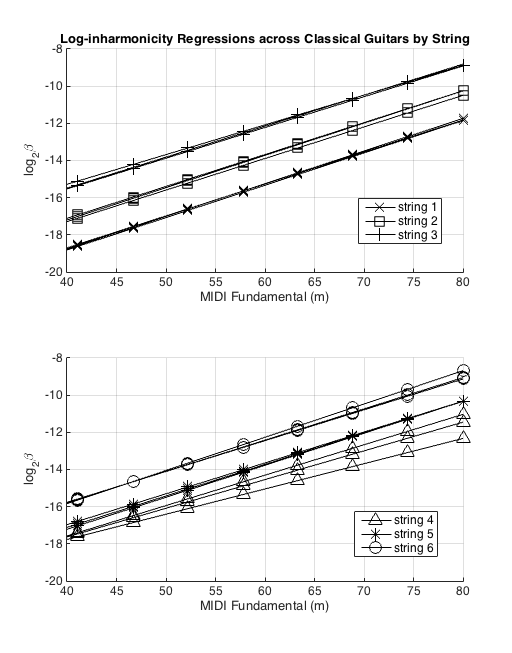
\includegraphics[scale=0.75]{traj-compare-cg}
\caption{Superimposed string-wise regressions of all three RWC classical guitars. Top: strings 1, 2, and 3. Bottom: strings 4, 5, and 6. Separated for visibility. Axes scales identical for comparison. Observe the consistent placement and orientation despite varying guitar.}
\end{figure}

\begin{figure}[!htbp] 
\label{fig:traj-compare-ag}
\centering
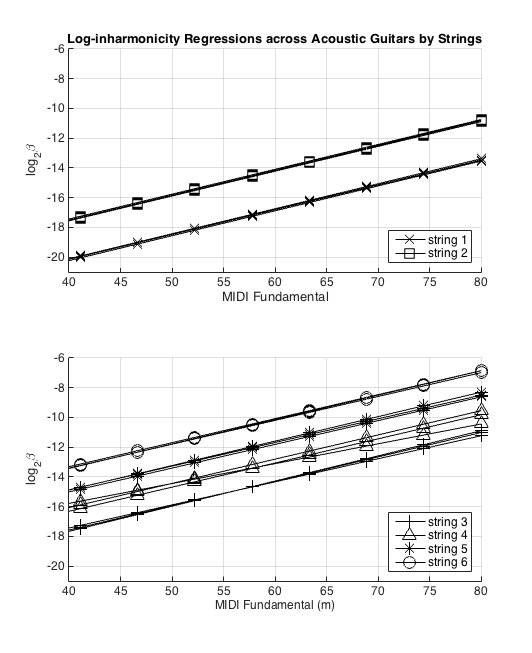
\includegraphics[scale=0.75]{traj-compare-ag}
\caption{}
\end{figure}

\begin{figure}[!htbp] 
\label{fig:traj-compare-eg}
\centering
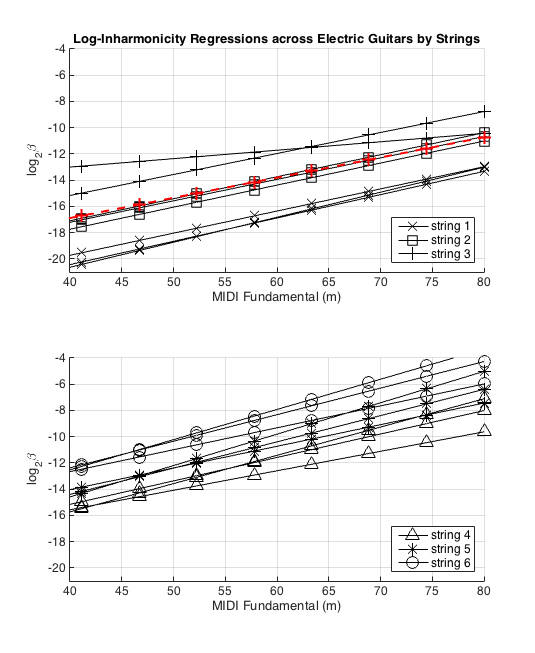
\includegraphics[scale=0.75]{traj-compare-eg}
\caption{}
\end{figure}

\begin{table}
\begin{center}
\begin{tabular}{|c||c|c|c|c|c|c|}
\hline
& \multicolumn{6}{|c|}{Classification} \\
\hline
Truth &1	&2	&3	&4	&5	&6\\
\hline
\hline
1	&\bf{0.92}	& 0.08	& 0	& 0	&0	& 0 \\ 
\hline
2	&0	& \bf{0.92}	& 0.08	& 0	&0	& 0 \\
\hline
3	&0	& 0.08	& \bf{0.38}	&0.54	& 0	& 0 \\ 
\hline
4	&0	& 0	& 0.08	&\bf{0.62}	& 0.30	& 0 \\
\hline
5	&0	& 0	& 0	&0	& \bf{0.77}	& 0.23\\ 
\hline
6	&0	& 0	& 0	&0	&0	& \bf{1.00} \\
\hline
\end{tabular}
\caption{Confusion matrix for one classification trial with EG131. Strings 3 and 4, as they are here, were frequently misclassified because of their regressions' poor discriminability.} 
\label{tab:cf-eg}
\end{center}
\end{table}

Further analysis revealed that inconsistent inharmonicity estimates were responsible for the electric guitars' regression variability. We examined the quality of fit of string regressions obtained from all recordings of each of the 3 guitars from each of the 3 types, and found that the classicals' and acoustics' range of determination coefficients was substantially smaller than the electrics'. Regressions for CG091, AG111, and EG131 are shown in Figure~\ref{fig:best-worst-r2} as an example of this; CG091's and AG111's best and worst strings' $r^2$ coefficients differ by only about one-hundredth, but the $r^2$ difference for EG131 is an enormous $0.87$.

\begin{figure}[!htbp] 
\label{fig:best-worst-r2}
\centering
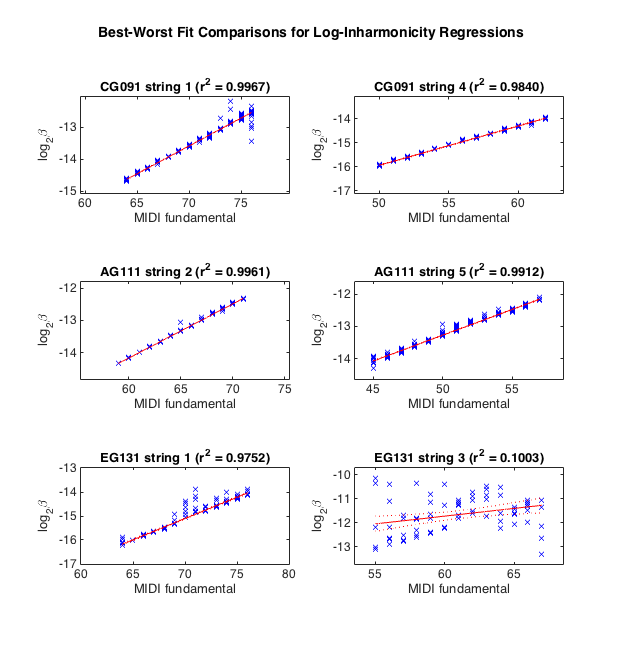
\includegraphics[scale=0.75]{best-worst-r2}
\caption{}
\end{figure}

Speculating why this might be the case, we wondered if the transduction of the EG pickups somehow played a role in obscuring reliable inharmonicity estimation -- either through their transfer function, possible noise introduction, or some non-linear characteristic. If this were the case, it would follow that higher-intensity performances would engage with the obscuring pickup phenomenon to a greater extent and produce measurably more variable inharmonicity estimates than lower-intensity performances. Since one of the RWC musicality parameters that varies for each featured guitar is dynamic level of the performance, we were able to separate "forte" and "piano" performances of the same guitar and analyze this interaction between degree of pickup transduction and inharmonicity estimation variability. For each guitar, and for each string, we collected note performances by common dynamic levels (piano, mezzo, and forte) and regressed their log-inharmonicities against their fundamentals, as usual. We then plotted statistics of the log-inharmonicities' residuals against their string's regression. Figure~\ref{fig:eg1-string-dyn} illustrates these statistics for EG131; other electric guitars are omitted because their statistics were similar.
\begin{figure}[!htbp] 
\label{fig:eg1-string-dyn}
\centering
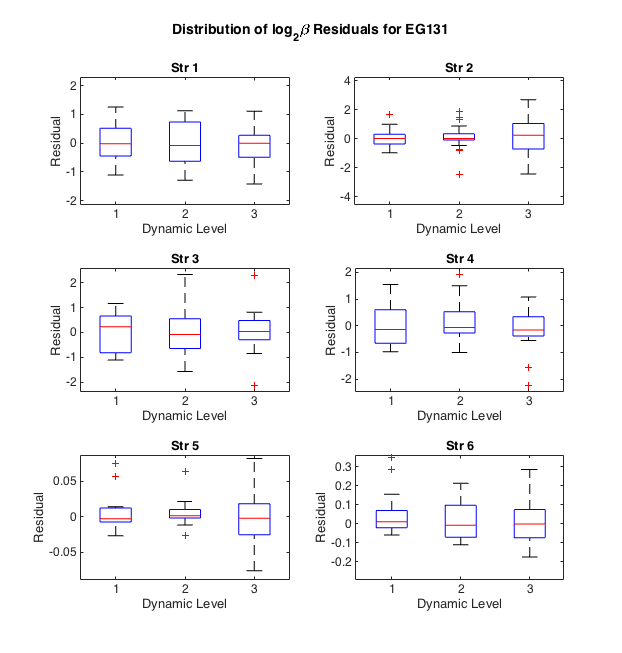
\includegraphics[scale=0.75]{eg1-string-dyn}
\caption{Boxplots of log-inharmonicity regression residuals for EG131 by dynamic level. Group 1: piano, Group 2: mezzo, Group 3: forte. Red center horizontal lines are medians; top and bottom edges of blue boxes represent upper and lower quartiles; whiskers depict full range of data excluding outliers; red plus signs denote outliers. Vertical axes not constant throughout plots; we're highlighting relative distributions of the boxplots here.}
\end{figure} 
We expected that variability would increase with dynamics, but unfortunately the data didn't support this hypothesis. Interquartile ranges didn't exhibit any clear trend with respect to performance intensity, nor was the magnitude of their variation noteworthy. The cause of the inharmonicity unreliability is therefore probably linked to some spectral characteristic of the electric guitars, e.g. considerably more non-tonal peaks which the MAT algorithm erroneously selects as partials, or some aspect of the pickup's frequency response that's throwing off the MAT algorithm, etc.





\section{Threats to Validity}
It's important to highlight factors that potentially undermine the claims of this work. Our system currently operates only on clean (i.e. no effects processing), isolated, monophonic guitar recordings, which are obviously not representative of the majority of guitar audio. Multiple layers of effects processing are commonly used by performers of the instrument to achieve distinctive, creative sounds. Guitarists often play in concert with other musicians, and frequently aren't the focal point of the song, buried in their companion's soundscapes. Moreover, guitar passages are rarely in their entirety strictly monophonic. It should be noted that these are large obstacles that separate our RWC subset from actual guitar performances, and thus the implications of our transcription results should be considerably tempered. Noteworthy though, is the extent to which other teams have overcome some of these factors. Barbancho, Abesser, Kehling, and Dittmar have implemented polyphonic capabilities into their systems with good success, so polyphony is perhaps a smaller barrier than the others. Maezawa's system achieved modest performance on RWC recordings that featured guitar passages combined with backing tracks.

Additionally, we assumed perfect fundamental pitch estimation in this work. Our decision to simply use the RWC labels stemmed from convenience and scope; the focus of this work was simply evaluation of a specific approach to examining notes' inharmonicities for tablature transcription, and having not to worry about the reliability of a pitch detection routine certainly expedited this thesis. That being said, it should be acknowledged that the reliability of one's pitch estimator is a sure factor in the translation of this work's results to the real world.

Furthermore, the MAT inharmonicity estimation routine we used was different from Barbancho's. The credibility of the comparison between our results and theirs is thus somewhat compromised. It's quite possible that any performance gains observed in our implementation are due in part to potentially superior inharmonicity extraction. This is, unfortunately, a factor we didn't control for, and if time had allowed we should have replicated Barbancho's system and substituted their inharmonicity estimation step with MAT to produce results that were as comparable as possible.





\section{Future Work}
A potential area for run-time performance enhancement for tablature transcription systems is the use of musical context. Musical passages on the guitar tend to exhibit continuity; it's usually the case that a riff is played in a localized area of the fretboard, for example, instead of jumping around the length of the guitar neck. It's empirically more natural for a performer to be motion conservative in this sense, as it's easier to play more notes quicker and it the piece sounds more uniform. Transcription systems could apply these performance-borne simplifications to their output to potentially improve accuracy, say, when a stray note is transcribed a plausible twelve frets away from the rest of those in the riff.

Necessary to do this, though, is a measure of objective confidence in the transcription. Without this, there'd be no way to determine whether it was the stray note or the majority of the riff which was correctly transcribed. We investigated the amenability of our log-inharmonicity residual-minimizing classification scheme to reliable confidence measurements, and reassuringly found encouraging results. Figure~\ref{fig:p-correct-res} displays the probability, for each of the nine RWC guitars, of our system producing a correct fretboard transcription given increasingly wide windows in which we consider a note's inharmonicity estimate to have fallen. The inverse trend between residual window width and correctness probability shows that we can reliably infer some degree of confidence in a note's transcription. This can be leveraged in a post-processing stage to further refine tablature with isolated erroneous, yet plausible, transcriptions.

Another dimension we didn't consider was varying the regression polynomial. It would be interesting to see how differently, if at all, the system would perform if the log inharmonicity transformation was forgone and an exponential fit was explored instead. Perhaps the ratio between inharmonicity estimation noise and the exponentials' residuals would be appreciably different to affect some change in the transcription results. This should be investigated in future inharmonicity-based transcription research.

\begin{figure}[!htbp] 
\label{fig:p-correct-res}
\centering
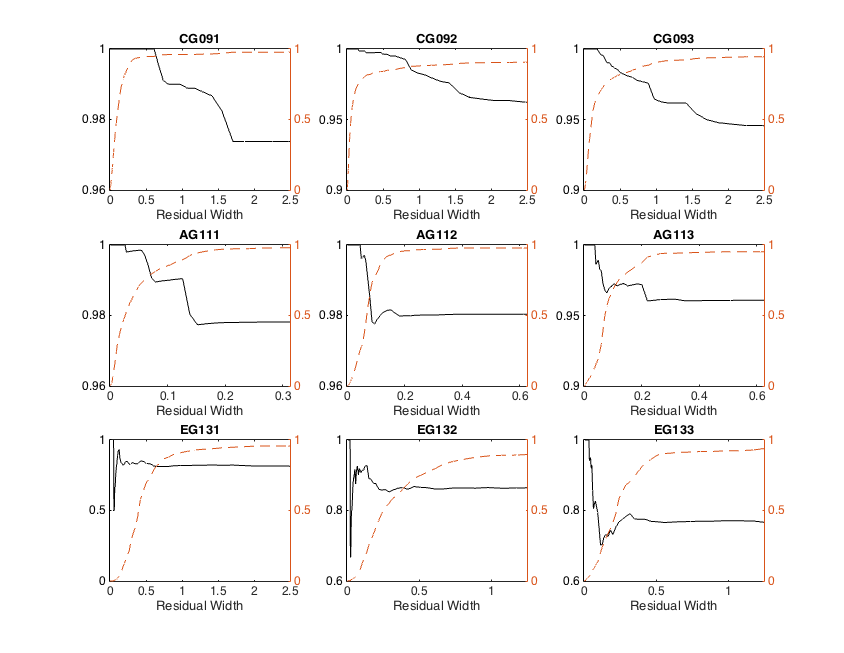
\includegraphics[angle=90,scale=0.65]{p-correct-res}
\caption{Solid black lines: probability of correctly transcribing a note given the residual width under which the note's log-inharmonicity falls, measured by the left-hand-side vertical axes. Dashed orange lines: CDF of the log-inharmonicity residuals, measured by the right-hand-side vertical axis.}
\end{figure} 

%The basic transcription results obtained in the previous chapter are modest; we achieved overall transcription accuracies of 43\%, 71\%, and 62\% for the RWC classical, acoustic, and electric guitars respectively. These accuracies don't tell the whole story, though. Closer inspection of Tables~\ref{tab:resultsRWC} and~\ref{tab:resultsTune} reveals that performance is heavily string-dependent. We can achieve a 0.93 F1-measure for string 6 (the electric guitar), but our worst-case F1-measure for string 3 is a disappointing 0.07 (also for the electric guitar). This is likely due to the somewhat overlapping inharmonicity trajectories of the inner strings, i.e. string 3 through 5 mainly, which is discussed further below when we consider factors that may have weakened system quality. This disparity between string-wise F1-scores suggests that in its current state, our system is more appropriate for tablature transcription of the "outer" strings, i.e. mainly strings 1, 2, and 6.

%Comparing these results to Barbancho's~\cite{barbanchoi2012} state-of-the-art inharmonicity-based transcription system, we see that average transcription accuracies of 98.3\%, 100\%, and 99.6\% are attainable. Though if we consider their performance when using inharmonicity coefficients averaged by guitar type (instead of those of each specific guitar), their performance slightly degrades to 96\%, 89.3\%, and 74\% mean accuracy. Comparison of our system with these poorer accuracies is actually fair, since we also use inharmonicity regressions obtained from averages over all guitars in each type.

%Still, our system's performance is lacking, and various factors could have contributed to this. Inconsistent inharmonicity estimation was likely the largest obstacle to greater performance. Sometimes our estimation routine would easily locate the inharmonic partials in the spectrum to produce a reliable estimate. But often it wouldn't, locating spurious spectral peaks that would corrupt the partials deviations calculation, which would subsequently corrupt the polynomial fit from which the inharmonicity estimate was derived. This variability in our system was somewhat mitigated when performing the inharmonicity regressions across many guitar recordings, effectively averaging it out, but no such averaging was in place for estimating inharmonicity of a single note. In this way, the sequential note-by-note transcription task challenged our system. 

%Additionally, the inharmonicity trajectories of the inner strings often intersected. This was a problem for our system, since our string classification mechanism was simply distance-minimization between the unknown note's inharmonicity and the observed inharmonicity trajectories. Notes with estimated inharmonicities residing close to that intersection would yield unpredictable assignments to either string. Clearly, even with flawless inharmonicity estimation, our transcription accuracy would have been limited.

%Results from the tuning compensation experiment are encouraging. Despite the inharmonicity estimation variability, we see that appropriately scaling the inharmonicity trajectories improves F1-score across the board by 17.5\% on average. Additionally, the individual string-wise F1-scores for all three tunings are non-decreasing after application of this scaling factor. In some cases, e.g. string 3 on the "WSD" tuning, drastic F1-score improvement from 0.11 to 0.45 occurs. This small experiment confirms this feature as a potential scope-widening addition to inharmonicity-based transcription systems, and justifies further investigation by other researchers with higher-accuracy implementations.

\noindent
\chapter{Conclusion}
We began by introducing the guitar and an essential component of its musicality: the overlapping pitch ranges of its strings. We related this to tablature and its ability to uniquely specify fretboard positions for musical passages, then highlighted its popularity and its tedious manual annotation process. This led us to introduce automatic transcription systems and their potential benefits for music students, and we reviewed previous work on this rich topic.

We paid special attention to Barbancho~\cite{barbanchoi2012}, who exploited only one feature known as inharmonicity in development of a successful tab transcription system using only audio. We explained how inharmonicity affects the degree of upward skew of a note's partials, then discussed the intuition behind its discriminative power before introducing our novel approach: characterizing strings as log-inharmonicity trajectories and regressions.

After reiterating one of Barbancho's key realizations -- that inharmonicity along a given string was deterministic -- we showed that the logarithm of these trajectories was linear with respect to MIDI pitch. We consequently proposed characterizing guitar strings by their log-inharmonicity lines and performing classification (and therefore implicitly, tablature transcription) by assigning to unknown notes the strings whose lines best approximated the notes' log-inharmonicities. Lastly, we derived the effect of a tuning change on these lines, and arrived at a general tuning-compensation feature applicable to any inharmonicity-based system.

Next, we introduced our experimental datasets -- a subset of the RWC music instruments database and a couple personal guitar recordings -- and outlined the experiments we conducted. We first performed benchmark comparisons against Barbancho's similar inharmonicity-based method, and then we assessed our tuning compensation feature's transcription performance for alternately-tuned guitars. Both evaluation areas were promising; our RWC tab transcription performance rivaled that of Barbancho's at 0.92, 0.94, and 0.79 for the classical, acoustic, and electric guitars respectively, while our average system accuracy on alternate-tuned guitars improved by 7\% compared to performance with no tuning compensation.

We wrapped up with a more detailed discussion of our experiment results, and an analysis of some of its less encouraging portions. A cursory investigation of the cause for the poorer electric guitar transcription performance revealed that it couldn't be the electric guitars' pickups that were responsible for impeding reliable inharmonicity estimation; it must rather be spectral nuances that confuse the inharmonicity estimation algorithm. We closed with limitations and future scope. More work should be done for a thorough appraisal of our system's merit, but results obtained thus far support the promise of our novel automatic tablature transcription approach.

%We introduced an additional inharmonicity-based approach to guitar string classification and tablature transcription, based on characterizing guitar strings' inharmonicity trajectories with linear regressions against pitch. Classification is performed by assigning to an unknown note the index of the trajectory which best explains the note's inharmonicity. We reported transcription F1-score performance of $0.43$, $0.71$, and $0.62$ for classical, acoustic, and electric guitars in the RWC dataset. 

%A tuning compensation feature was also proposed and analyzed. We derived that a deviation from standard tuning could be accounted for in our regressions with a scaling factor on the deviant strings' trajectories. To test this, we recorded an electric guitar in standard, "dadgad", whole-step up, and whole-step down tunings, and performed classification both with and without tuning compensation. With our modification, our F1-scores improved by 17.5\% on average for the three tunings we investigated.

%Our system falls short of other inharmonicity-based transcription methods, though we suspect this is largely due to poor internal inharmonicity estimation. Encouragingly, our tuning compensation feature improved performance on alternate-tunings, and should be investigated by other researchers with higher-accuracy transcription systems. Future work should explore other polynomial regressions that more closely match theoretical inharmonicity trajectories. Additionally, performance assessment on polyphonic inputs is requisite for a more thorough appraisal of this system's merit.

%\appendix
%\include{appendix}

\backmatter

%\renewcommand{\baselinestretch}{1.0}\normalsize

% By default \bibsection is \chapter*, but we really want this to show
% up in the table of contents and pdf bookmarks.
\renewcommand{\bibsection}{\chapter{\bibname}}
%\newcommand{\bibpreamble}{This text goes between the ``Bibliography'' header and the actual list of references}
\bibliography{mybib} %your bib file
\bibliographystyle{plainnat}


\end{document}
